\documentclass[tikz,border=10pt]{standalone}
\usepackage{tikz}
\usetikzlibrary{arrows.meta,automata,positioning,shapes}

\begin{document}

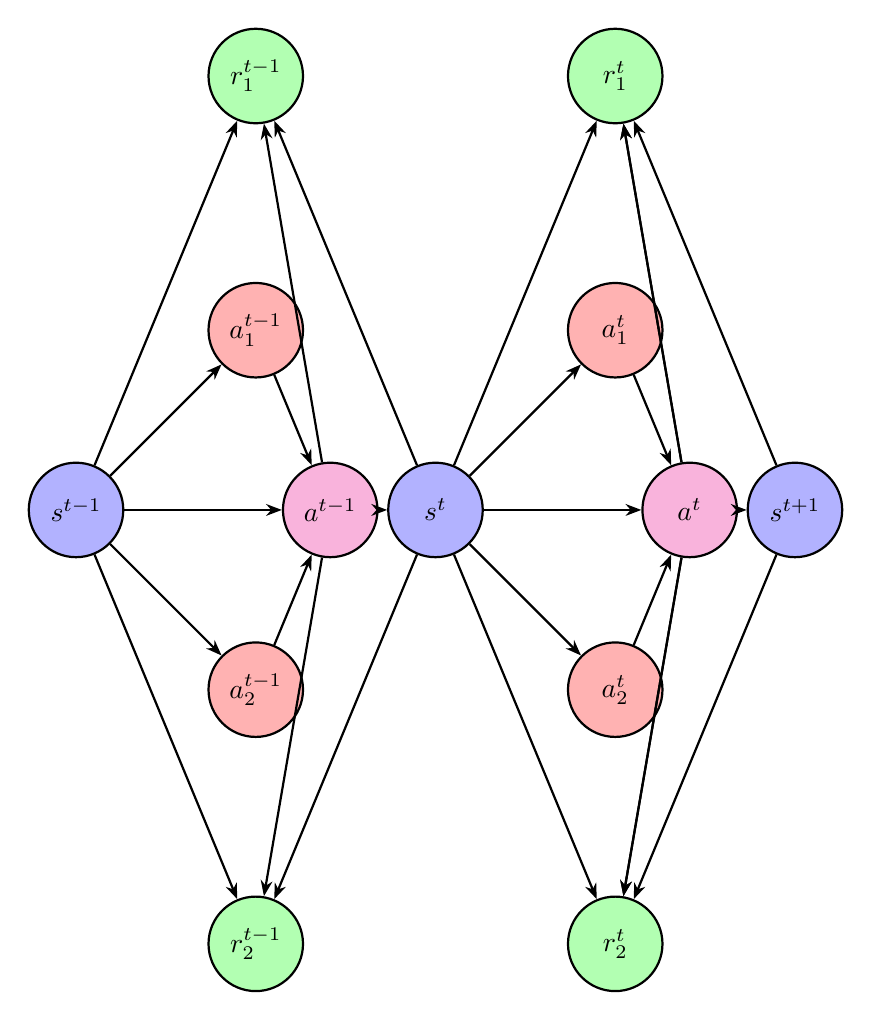
\begin{tikzpicture}[->, >={Stealth[length=2mm]}, node distance=2cm, thick, main/.style = {draw, circle, minimum size=1.2cm, align=center}]
  % Nodes for Agent 1
  \node[main, fill=blue!30] (s_t1) {\(s^{t-1}\)};
  \node[main, fill=red!30] (a1_t1) [above right=of s_t1] {\(a_1^{t-1}\)};
  \node[main, fill=blue!30] (s_t) [below right=of a1_t1] {\(s^t\)};
  \node[main, fill=red!30] (a1_t) [above right=of s_t] {\(a_1^t\)};
  \node[main, fill=blue!30] (s_t2) [below right=of a1_t] {\(s^{t+1}\)};

  % Nodes for Agent 2
  \node[main, fill=red!30] (a2_t1) [below right=of s_t1] {\(a_2^{t-1}\)};
  \node[main, fill=red!30] (a2_t) [below right=of s_t] {\(a_2^t\)};

  % Rewards for Agent 1
  \node[main, fill=green!30] (r1_t1) [above=of a1_t1] {\(r_1^{t-1}\)};
  \node[main, fill=green!30] (r1_t) [above=of a1_t] {\(r_1^t\)};

  % Rewards for Agent 2
  \node[main, fill=green!30] (r2_t1) [below=of a2_t1] {\(r_2^{t-1}\)};
  \node[main, fill=green!30] (r2_t) [below=of a2_t] {\(r_2^t\)};

    %Join Actions
    \node[main, fill = magenta!30] (a_t1) [right=of s_t1] {\(a^{t-1}\)};
    \node[main, fill = magenta!30](a_t) [right=of s_t] {\(a^{t}\)};
  % Ellipses nodes
  % \node (left_dots) [left=of s_t1] {\(\ldots\)};
  % \node (right_dots) [right=of s_t2] {\(\ldots\)};

  % Paths for Agent 1
  \path 
        (s_t1) edge (a1_t1)
        (s_t1) edge (a_t1)
        (a_t1) edge (s_t)
        (a1_t1) edge (a_t1)
        (s_t) edge (a1_t)
        (a1_t) edge (a_t)
        (a_t1) edge (r1_t1)
        (s_t1) edge (r1_t1)
        (s_t) edge (r1_t1)
        (a_t) edge (r1_t)
        (s_t) edge (r1_t)
        (s_t2) edge (r1_t) 
        (a_t) edge (r1_t);

  % Paths for Agent 2
  \path 
        (s_t1) edge (a2_t1)
        (a2_t1) edge (a_t1)
        (s_t) edge (a2_t)
        (s_t) edge (a_t)
        (a2_t) edge (a_t)
        (a_t) edge (s_t2)
        (a_t1) edge (r2_t1)
        (s_t1) edge (r2_t1)
        (s_t) edge (r2_t1)
        (a_t) edge (r2_t)
        (s_t) edge (r2_t)
        (s_t2) edge (r2_t)
        (a_t) edge (r2_t);

  % Joint actions to next states (hidden for simplification, can be added if needed)
  % \path (a1_t1) edge (s_t)
  %      (a2_t1) edge (s_t)
  %      (a1_t) edge (s_t2)
  %      (a2_t) edge (s_t2);

\end{tikzpicture}

\end{document}
